	\paragraph{QuizziPedia::Front-End::Directives::InfoQuestionnaireDirective}
		
		\label{QuizziPedia::Front-End::Directives::InfoQuestionnaireDirective}
		
		\begin{figure}[ht]
			\centering
			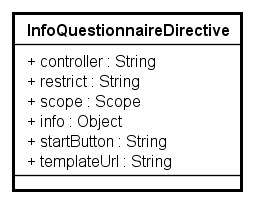
\includegraphics[scale=0.80,keepaspectratio]{UML/Classi/Front-End/QuizziPedia_Front-end_Templates_InfoQuestionnaireTemplate.png}
			\caption{QuizziPedia::Front-End::Directives::InfoQuestionnaireDirective}
		\end{figure} \FloatBarrier
		
		\begin{itemize}
			\item \textbf{Descrizione}: rappresenta il componente grafico che permette all'utente di visualizzare le informazioni principali del questionario che si sta per svolgere. Viene visualizzato dinamicamente all'interno della view FillingQuestionnaireView mediante il controller FillingQuestionsController;
			\item \textbf{Utilizzo}: viene utilizzato per consentire all'utente di visualizzare le informazioni principali del questionario che si sta per svolgere. Informazioni come:
			\begin{itemize}
				\item Nome del questionario;
				\item Nome dell'autore del questionario;
				\item Data di creazione del questionario;
				\item Argomento del questionario;
				\item Bottone per iniziare il questionario;
			\end{itemize}
			\item \textbf{Relazioni con altre classi}: 
			\begin{itemize}
				\item \textit{IN} \texttt{FillingQuestionnaireModelView}: classe di tipo modelview la cui istanziazione è contenuta all'interno della variabile di ambiente \$scope di \textit{Angular.js\ped{G}}. All'interno di essa sono presenti le variabili e i metodi necessari per il \textit{Two-Way Data-Binding\ped{G}} tra la view \texttt{FillingQuestionnaireView} e il controller \texttt{FillingQuestionnaireController};
				\item \textit{IN} \texttt{FillingQuestionsController}: questa classe permette di gestire la creazione e la modifica di una domanda a riempimento di spazi;
				\item \textit{IN} \texttt{LangModel}: rappresenta il modello delle informazioni per la giusta traduzione dell'applicazione.
			\end{itemize}
			\item \textbf{Attributi}: 
			\begin{itemize}
				\item \texttt{+ controller: String} \\ Stringa contenente il nome del controller della direttiva;
				\item \texttt{+ restrict: String} \\ Stringa che permette di definire le modalità di inserimento della direttiva all'interno della pagina;
				\item \texttt{+ scope: Scope} \\ Oggetto scope interno della direttiva, contiene:
				\begin{itemize}
					\item \texttt{+ info: Object} \\ Oggetto contenente tutte le informazioni sul questionario, ovvero:
					\begin{itemize}
						\item \texttt{name};
						\item \texttt{author};
						\item \texttt{date};
						\item \texttt{topic}.
					\end{itemize}
					\item \texttt{+ startButton: String} \\ Attributo che viene utilizzato per visualizzare la giusta traduzione della \textit{label\ped{G}} per il bottone di inizio del questionario selezionato, in italiano o in inglese; 
				\end{itemize}
				\item \texttt{+ templateUrl: String} \\ Stringa contenente il percorso del file \textit{HTML\ped{G}} che contiene la direttive.
			\end{itemize}
		\end{itemize}
		